\documentclass[conference]{IEEEtran}
\IEEEoverridecommandlockouts

\usepackage{graphicx}
\usepackage{amsmath,amssymb}
\usepackage{booktabs}
\usepackage{multirow}
\usepackage{url}
\usepackage{tikz}
\usetikzlibrary{positioning,arrows.meta}
\usepackage{algorithm}
\usepackage{algpseudocode}
\usepackage{float}

\begin{document}

\title{A Multi-Environment Marine Radar Dataset and Baseline for Inland and Coastal Small-Craft Autonomy}

\author{
\IEEEauthorblockN{JC~Vaught, Douglas~Cahl, and Yi~Wang}
\IEEEauthorblockA{Department of Mechanical Engineering\\
University of South Carolina, Columbia, SC, USA\\
Email: \{JVAUGHT, DCAHL\}@sc.edu, YIWANG@cec.sc.edu}
}

\maketitle

\begin{abstract}
Marine radar is a critical sensor for small craft and coastal autonomy, especially in poor visibility where cameras and LiDAR may fail. Despite widespread deployment of inexpensive solid-state marine radars, scalable datasets and tools for learning-based perception remain scarce, and collecting high-quality labels on radar imagery is costly. This paper targets this gap for inland and near-coastal waterways in the southeastern United States. 

We study object detection for small boats in marine radar imagery under a severe label budget. Models are first trained on the public RADAR3000 dataset of $3000$ labeled radar frames containing boat detections, then fine-tuned on a new canal-style dataset of $96$ labeled frames and $637$ annotated objects collected across lakes, rivers, and harbor scenes. In addition, we record $24\,988$ unlabeled frames across diverse locations, times of day, and weather conditions using a commercial Furuno NXT marine radar, and we introduce a family of open-source tools that make this type of data collection and processing reproducible: a radar-image annotator, a raw range--azimuth to PNG converter, and a synthetic echo-trail generator that constructs temporal context by overlaying transparent past sweeps.

We benchmark modern detector and segmentation architectures on the RADAR3000 boat-detection task, achieving up to 0.928 mAP@0.5 (YOLOv12-L, 1024 input) and 0.935 mAP@0.5 (MRISNET segmentation baseline). We also evaluate a self-supervised backbone pretraining stage that uses all available radar imagery (the $24\,988$ in-house unlabeled frames plus the $3000$ RADAR3000 frames) before standard supervised training. Finally, we demonstrate qualitative generalization to the Pohang Canal radar dataset without additional training. All software tools will be released to enable the community to scale marine radar data collection and experimentation, while the datasets themselves remain institutionally hosted due to access constraints.
\end{abstract}

\begin{figure}[t]
\centering
\includegraphics[width=\linewidth]{images_lidar_RGB-Radar_thermal/stacked_cropped_images_tikz.pdf}
\caption{Sensor modality comparison for maritime object detection: (a) RGB camera, (b) thermal camera, (c) LiDAR, and (d) radar from Pohang Canal Dataset~\cite{chung2023pohang_canal_dataset}. Marine radar excels in adverse weather (rain, fog, darkness) where cameras and LiDAR fail, making it critical for robust small-vessel autonomy in inland and coastal waters.}
\label{fig:modality_comparison}
\end{figure}

\section{Introduction}
Marine radar is a mature technology for navigation and collision avoidance, yet learning-based perception for radar imagery remains in its early stages compared to vision. Cameras dominate research on maritime object detection, while radar is often relegated to thresholding and hand-crafted tracking pipelines. For small vessels and near-shore autonomy, this imbalance is problematic. Radar remains effective in rain, fog, darkness, and high dynamic range conditions that challenge cameras, but modern data-driven models require curated datasets and tooling that have not been widely available for low-cost commercial marine radars. Recent surveys on radar perception for autonomous systems highlight this gap~\cite{zhou2022deep_radar_perception_sensors, srivastav2023radars_for_autonomous_driving_arxiv}.

This work focuses on small-vessel detection from plan-position-indicator (PPI) radar imagery in inland lakes, rivers, and near-coastal waters. Our target application is proof-of-concept autonomy and situational awareness for small craft operating in cluttered docks, marinas, and channels in the southeastern United States. In this setting, three constraints dominate system design. First, manual labeling of radar imagery is extremely expensive, and even experienced annotators struggle in dense clutter. Second, the variety of environments, traffic patterns, and range settings is large compared to the number of labeled examples that can be collected in early-stage projects. Third, the research community lacks an open, reproducible toolchain for converting raw range--azimuth radar data from inexpensive commercial units into model-ready images and annotations.

We address these constraints with a combination of pretraining on an existing public dataset, targeted annotation of a small canal-style dataset, and an integrated software toolchain for scaling data collection. We begin from the RADAR3000 dataset~\cite{kz258852_radar300_dataset_m_radar}, a public collection of $3000$ marine radar frames with boat annotations, which we treat as a generic source domain for boat detection through transfer learning~\cite{pan2010transfer_learning_survey}. We then collect a new dataset using a Furuno NXT solid-state radar installed on small vessels and shore-based mounts at multiple sites: three South Carolina lakes (Murray, Greenwood, Monticello), Portsmouth City Park on the Elizabeth River in Virginia, the Charleston harbor region via Grice Marine Lab and Demetre Park, and open-ocean conditions off Folly Beach. The labeled subset of this dataset currently contains $96$ frames with $637$ annotated objects in two classes (dynamic and static), while a larger unlabeled subset of $24\,988$ frames spans different times of day and weather conditions, including rain and high wind.

From a modeling perspective, we study whether pretraining detectors on RADAR3000 and then fine-tuning on the small canal dataset improves detection performance compared to training on the canal dataset alone. From a tooling perspective, we introduce and will release three components designed to make commercial marine radar data more accessible: (i) a radar image annotator tailored to PPI data and boat labels, (ii) a converter that transforms proprietary Furuno range--azimuth sweeps into $1735\times 1735$ PNG images suitable for deep learning, and (iii) a synthetic echo-trail generator that overlays transparent past sweeps under a fully opaque current sweep to create temporal context of configurable length.

\begin{figure}[t]
\centering
\includegraphics[width=\linewidth]{figures/fig01_radar_hardware.pdf}
\caption{Furuno DRS4DNXT 24\,in.\ solid-state Doppler X-band radome radar (MSRP \$3k) mounted on a tripod on the embankment. Low-cost control equipment (Raspberry Pi 5) is located below the radar and runs headless, minimizing cabling.}
\label{fig:radar_hardware}
\end{figure}

\begin{figure}[t]
\centering
\includegraphics[width=0.95\linewidth]{figures/sc_sites_map.pdf}
\caption{Geographic distribution of data collection sites in South Carolina. Inland sites (Lake Murray, Greenwood, Monticello) provide freshwater environments, while coastal and harbor sites (Charleston, Portsmouth(not pictured), Folly Beach) capture near-shore conditions and maritime traffic.}
\label{fig:collection_map}
\end{figure}

The main contributions can be summarized as follows in a single narrative. We assemble and describe a diverse inland and coastal marine radar dataset built around a small labeled canal subset and a much larger unlabeled corpus. We benchmark modern detector and segmentation architectures on RADAR3000 and describe transfer-learning regimes for adapting models to the small canal dataset, including self-supervised backbone pretraining on the unlabeled corpus. We design and implement an open-source software stack that transforms raw range--azimuth data from a low-cost Furuno NXT radar into annotated images with optional synthetic echo trails, enabling other groups to reproduce and scale similar data-collection efforts. Finally, we demonstrate that the resulting models generalize qualitatively to the Pohang Canal radar dataset~\cite{chung2023pohang_canal_dataset} without retraining, illustrating the potential of this approach for cross-dataset transfer.

The remainder of the paper builds up from data and tools to models and results. Section~\ref{sec:data} describes RADAR3000, the new canal dataset, and the unlabeled corpus. Section~\ref{sec:acq} details the radar hardware, raw data format, and conversion and echo-trail processing. Section~\ref{sec:models} presents the chosen detector architectures and training protocols. Section~\ref{sec:toolchain} describes the open-source toolchain. Section~\ref{sec:setup} outlines the experimental setup, followed by quantitative and qualitative results in Section~\ref{sec:results}. Section~\ref{sec:discussion} discusses limitations and connections to classical radar-processing techniques such as CFAR and ST-DBSCAN, and Section~\ref{sec:conclusion} concludes with future directions, including scaling to millions of frames by mid-2026.

\section{Datasets}
\label{sec:data}
This section describes the datasets used in this work. We rely on one public marine radar dataset for pretraining, a small labeled canal-style dataset for evaluation and fine-tuning, a larger unlabeled corpus that primarily supports future semi-supervised work, and an external dataset used purely for qualitative generalization figures.

\subsection{RADAR3000}
RADAR3000 is a public marine radar dataset containing $3000$ PPI radar frames with boat annotations. Each frame is labeled in a single foreground class denoted by the label ``B'' for boat. In total, the dataset contains $3000$ boat instances, suggesting that the majority of frames contain a single annotated boat, though this is not a strict requirement. The imagery is provided in a format compatible with standard object-detection frameworks, and prior work has explored its use for YOLO-style detectors.

In our experiments, RADAR3000 serves both as a benchmark for modern marine-radar models and as a source dataset for transfer learning. We treat its single boat class as compatible with the dynamic-boat class in our canal dataset and use it to initialize weights for modern one-stage detectors. The precise split of RADAR3000 into training, validation, and testing subsets can follow the original dataset recommendation or, when not specified, a conventional division such as $80$~\% training and $20$~\% validation. RADAR3000 performance is reported both as a standalone benchmark and to confirm that pretraining has converged before transfer to the canal dataset.

\begin{figure}[t]
\centering
\includegraphics[width=\linewidth]{latex_figures/radar3000_clean_tikz.pdf}
\caption{Sample detections from the RADAR3000 public dataset, showing labelled boat detection from a stationary radar.}
\label{fig:radar300_samples}
\end{figure}

\subsection{USC Canal Radar Dataset}
The new labeled dataset introduced in this work is a canal-style marine radar dataset collected using a Furuno NXT radar between May~2025 and December~2025. Data collection covers several inland lakes and near-coastal environments in the southeastern United States and Virginia, including Lake Murray, Lake Greenwood, Lake Monticello, Portsmouth City Park on the Elizabeth River, the Charleston harbor region near Grice Marine Lab and Demetre Park, and open-ocean conditions off Folly Beach. Environmental variability includes rain, nighttime, early morning, mid-day, and windy conditions, but no snow at present. Individual data-collection sessions last up to approximately two hours at a time.

The currently labeled subset contains $96$ frames with a total of $637$ annotated objects. Annotations are divided into two classes. The first class, dynamic, corresponds to moving boats and other actively maneuvering targets. The second class, static, covers moored boats, piers, and other non-moving or quasi-static objects that are relevant for navigation but exhibit different radar signatures and dynamics. The choice of a two-class scheme reflects a compromise between annotation cost and the need to separate moving targets from persistent clutter.


\begin{figure}[t]
\centering
\includegraphics[width=\linewidth]{latex_figures/house_dataset_samples_zoomed.pdf}
\caption{2x zoomed central region samples from six radar frames with synthetic echo trails ($T=10$). Collection sites: Murray Dam, Grice Lab, Folly Beach, Portsmouth City Park, Lake Monticello, Greenwood Park.}
\label{fig:house_dataset_samples}
\end{figure}

The unlabeled portion of the dataset currently contains $24\,988$ frames. These frames share the same acquisition hardware and environmental diversity as the labeled subset but have not yet been manually annotated. They are intended for self-supervised and semi-supervised learning experiments, as well as for scaling models when annotation resources permit. For this paper, the unlabeled frames are used implicitly via echo-trail generation when temporal context spans multiple sweeps, but no explicit pseudo-labeling is performed.

To make the structure of the datasets concrete, Table~\ref{tab:datasets} summarizes the key properties of RADAR3000 and the USC canal dataset, including frame counts, labeled object counts, number of classes, and intended usage. Entries marked with placeholders can be updated once final splits and statistics are computed.

\begin{table}[t]
\centering
\caption{Datasets used in this work. Counts for splits marked with an asterisk are placeholders to be finalized.}
\label{tab:datasets}
\resizebox{\columnwidth}{!}{%
\begin{tabular}{lcccc}
\toprule
Dataset & Frames & Labeled & Classes & Primary Use \\
\midrule
RADAR3000 & $3000$ & $3000$ obj. & $1$ (boat) & pretraining \\
USC-Canal-Labeled & $96$ & $637$ obj. & $2$ (dyn, stat) & fine-tune, test \\
USC-Canal-Unlabeled & $24\,988$ & $0$ & -- & self-supervised \\
Pohang-Subset & $N_{\text{P}}^\ast$ & $M_{\text{P}}^\ast$ & $C_{\text{P}}^\ast$ & generalization \\
\bottomrule
\end{tabular}%
}
\end{table}

\begin{figure}[t]
\centering
\includegraphics[width=\linewidth]{python_figures/fig06_dataset_comparison.png}
\caption{Dataset comparison showing visual differences between RADAR3000 (left, cleaner with less clutter) and USC Canal (right, more cluttered inland environment). This distribution shift motivates the use of pretraining and fine-tuning rather than training only on the small canal dataset.}
\label{fig:dataset_comparison}
\end{figure}

\begin{figure}[t]
\centering
\includegraphics[width=\linewidth]{/Users/jacobvaught/Downloads/Classes/Fall 2025/Conf_Papers/IEEE Papers/one_click_annotation_paper/latex_figures/fig08_temporal_aggregates_pgfplots.pdf}
\caption{Temporal distribution of the $24\,988$ unlabeled frames. Top-left: frames by hour of day. Top-right: frames by day of week. Bottom-left: cumulative frames over time (month ticks). Bottom-right: collection intensity heatmap by hour and month (warmer colors indicate higher frame density).}
\label{fig:temporal_coverage}
\end{figure}

\subsection{Pohang Canal Dataset for Qualitative Generalization}
The Pohang Canal radar dataset~\cite{chung2023pohang_canal_dataset} is an external dataset collected in a Korean canal environment and has been used in prior maritime perception work. In this paper, we do not use Pohang images for training or validation. Instead, a small subset is reserved for generating qualitative figures that illustrate how models trained on RADAR3000 and the USC canal dataset behave under distribution shift. The experimental protocol is simple: detectors trained on our training sets are applied to Pohang Canal radar frames without further fine-tuning, and their predictions are visualized alongside any available annotations. This provides an intuitive sense of cross-dataset generalization without affecting the main quantitative conclusions.

\begin{figure}[t]
\centering
\includegraphics[width=\linewidth]{python_figures/fig09_pohang_preview.png}
\caption{Preview of the Pohang Canal dataset, showing samples from a Korean canal environment with different radar hardware and traffic patterns. Used for qualitative cross-dataset generalization testing without retraining.}
\label{fig:pohang_preview}
\end{figure}

\section{Radar Acquisition and Preprocessing}
\label{sec:acq}
The USC canal dataset is built around a low-cost commercial marine radar with a proprietary raw data format. This section describes the hardware, the raw data layout, and the conversion into model-ready PNG images. It also introduces the synthetic echo-trail augmentation mechanism used to provide temporal context.

\subsection{Hardware and Operating Modes}
All data for the USC canal dataset are collected using a Furuno NXT radar, a solid-state marine radar commonly deployed on small recreational and research vessels. The radar is operated as a cheap commercial unit with default resolution settings and varying range scales up to approximately $3$ nautical miles. This variability in range settings is a distinctive aspect of the dataset and introduces a wider diversity of spatial scales than in many fixed-configuration datasets.

The radar antenna rotates at rates between $24$ and $48$ revolutions per minute, with occasional runs at $30$~rpm. Most experiments use data collected at $24$ or $48$~rpm, and future work will standardize on $48$~rpm to simplify temporal modeling and trajectory estimation. Each full rotation produces a sweep of raw radar returns over angle, which are stored along with metadata such as range setting and timestamp.

\subsection{Raw Range--Azimuth Format and Quantization}
The raw data from the Furuno radar are stored as range--azimuth samples per sweep. For each antenna angle, the sensor reports a fixed number of range bins. In the current configuration, each sweep contains $868$ range bins per azimuth angle and between $600$ and $1000$ distinct azimuth angles (or pulses) per rotation, depending on rotational speed and vendor settings. This yields a polar grid of complex-valued or magnitude-only radar returns.

Although vendor documentation advertises $8$~bit amplitude resolution, direct inspection of the raw data reveals an effective $4$~bit quantization with an additional zero level. Intensities are therefore represented with $16$ distinct non-zero levels plus a background level, which has implications for dynamic range and noise modeling. In this work, we operate on magnitude values and defer more sophisticated complex-valued processing and calibration to future signal-processing papers.
	
\subsection{Conversion to PNG Images}
To make the data compatible with common deep-learning frameworks, each polar sweep is projected into a square $1735\times 1735$ image. The dimension is chosen so that the $868$ radial bins can be mapped approximately one-to-two with interpolation into a square Cartesian grid covering the maximum range used in the dataset, while the angular dimension determines the sampling around the circle.

The conversion process consists of three steps. First, the polar range--azimuth grid is interpolated onto a Cartesian $x$--$y$ grid centered at the radar location using a simple nearest-neighbor or bilinear scheme. Second, the $4$~bit quantized magnitudes are mapped into an 8-bit grayscale intensity range, with optional contrast stretching to emphasize relevant returns. Third, the resulting grayscale image is optionally color-mapped using standard colormaps for visualization but stored internally as a single-channel PNG for training.

\begin{figure}[t]
\centering
\includegraphics[width=\linewidth]{python_figures/fig13_conversion_pipeline.png}
\caption{Conversion pipeline from raw polar range--azimuth data to training-ready PNG images. Four stages: (1) raw Furuno sweep, (2) polar-to-Cartesian interpolation, (3) quantization and intensity mapping, (4) normalized 1735×1735 PNG output with metadata recording.}
\label{fig:conversion_pipeline}
\end{figure}

\begin{figure}[t]
\centering
\includegraphics[width=\linewidth]{latex_figures/fig10_range_variability.pdf}
\caption{Range setting variability: same scene at 0.125\,nm, 0.25\,nm, and 0.5\,nm scales (gain level 50). Spatial resolution and apparent object size vary with range, requiring models to handle multi-scale objects and diverse spatial sampling.}
\label{fig:range_variability}
\end{figure}

At this stage, we deliberately avoid heavy preprocessing such as constant false alarm rate (CFAR) thresholding~\cite{rashid2025cfar_sar_vessels}, entropy-based enhancement, or radar high dynamic range (HDR) compression. Those techniques are the focus of separate, more signal-processing-oriented papers and undergraduate projects. For the present work, the primary transformation is from raw polar data to a simple, consistent Cartesian image representation that can be used with standard object detectors.

\subsection{Synthetic Echo-Trail Generation}
Radar echo trails provide temporal context by displaying residual echoes from past sweeps under the current sweep. In conventional marine radar displays, echo trails can help human operators perceive motion and distinguish moving targets from static clutter. Inspired by this, we implement a synthetic echo-trail generator that overlays a configurable number of past frames behind the current frame.

Given a sequence of PNG images corresponding to consecutive radar sweeps, the echo-trail generator constructs a composite image by assigning decreasing transparency to older frames and rendering the latest frame fully opaque. Multiple trail lengths are supported and are treated as data augmentation. For example, a trail length of $T=4$ uses the current frame and the three preceding frames; a trail length of $T=16$ uses a much longer temporal window. Trails may include both past and future frames relative to the labeled frame when labels are associated with a specific sweep; however, in this paper we restrict to past sweeps for simplicity.

The basic algorithm for echo-trail generation can be expressed succinctly as follows.

\begin{algorithm}[t]
\caption{Synthetic Echo-Trail Generation}
\label{alg:echo}
\begin{algorithmic}
\State Input: sequence of grayscale images $I_{t-T+1}, \dots, I_{t}$, trail length $T$, opacity schedule $\alpha_{1} \leq \dots \leq \alpha_{T-1} < \alpha_{T}=1$
\State Initialize composite image $C \gets 0$
\For{$k \gets 1$ to $T$}
  \State $C \gets C + \alpha_{k} \cdot I_{t-T+k}$
\EndFor
\State Optionally clip $C$ to valid intensity range
\State Output composite echo-trail image $C$
\end{algorithmic}
\end{algorithm}

In practice, the opacity schedule can be chosen as a simple linear ramp or an exponential decay. For example, a linear schedule might set $\alpha_{k} = k/T$, while an exponential schedule might use $\alpha_{k} = \beta^{T-k}$ for some $\beta \in (0,1)$. The generator is applied on-the-fly during training so that a single labeled frame can yield multiple augmented inputs with different trail lengths and opacity schedules. This effectively increases the apparent dataset size and allows the detector to exploit motion cues without explicit tracking.

\begin{figure}[t]
\centering
\includegraphics[width=\linewidth]{python_figures/fig15_echo_trail_generation.png}
\caption{Echo-trail generation process: (top row) four individual frames (T, T-1, T-2, T-3) with boat in different positions, (middle row) same frames with decreasing opacity, (bottom left) final composite echo-trail image (T=4) showing ghosted boat trajectory, (bottom right) pseudocode for the echo-trail algorithm.}
\label{fig:echo_trail_generation}
\end{figure}

\begin{figure}[t]
\centering
\includegraphics[width=\linewidth]{python_figures/fig16_echo_trail_variants.png}
\caption{Echo-trail length variants: T=1 (baseline, single frame) vs.\ T=4, T=8, T=16. Longer trails provide more temporal context but introduce ghosting and blur. Optimal trail length balances motion perception against computational cost.}
\label{fig:echo_trail_variants}
\end{figure}

\begin{figure}[t]
\centering
\includegraphics[width=\linewidth]{python_figures/fig17_motion_visualization.png}
\caption{Motion visualization: (left) individual frames showing boat trajectory with position markers, (right) echo-trail composite with full trajectory overlay and velocity vector. Motion cues emerge naturally from layered sweeps without explicit velocity estimation.}
\label{fig:motion_visualization}
\end{figure}

Figure~\ref{fig:pipeline} illustrates the end-to-end processing pipeline from raw data to detector input, including echo-trail generation.

\begin{figure}[t]
\centering
\resizebox{\columnwidth}{!}{%
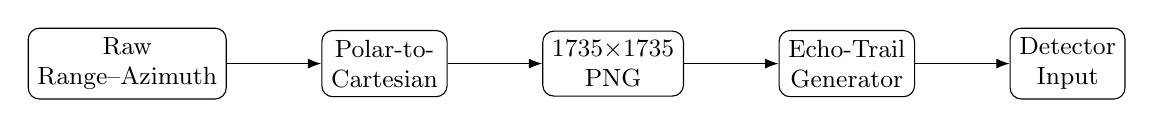
\begin{tikzpicture}[node distance=1.2cm, >=Latex]
\node[draw, rectangle, rounded corners, align=center, font=\small] (raw) {Raw\\Range--Azimuth};
\node[draw, rectangle, rounded corners, right=of raw, align=center, font=\small] (cart) {Polar-to-\\Cartesian};
\node[draw, rectangle, rounded corners, right=of cart, align=center, font=\small] (png) {$1735{\times}1735$\\PNG};
\node[draw, rectangle, rounded corners, right=of png, align=center, font=\small] (trail) {Echo-Trail\\Generator};
\node[draw, rectangle, rounded corners, right=of trail, align=center, font=\small] (det) {Detector\\Input};

\draw[->] (raw) -- (cart);
\draw[->] (cart) -- (png);
\draw[->] (png) -- (trail);
\draw[->] (trail) -- (det);
\end{tikzpicture}%
}
\caption{Processing pipeline from raw range--azimuth radar data to detector input, including synthetic echo-trail generation.}
\label{fig:pipeline}
\end{figure}

\section{Detectors and Training Protocols}
\label{sec:models}
This section describes the object-detection architectures and training protocols used in the experiments. Because the primary focus of this paper is on pretraining, fine-tuning, and tooling rather than novel network architectures, we select widely used models with strong performance in general object detection and adapt them to radar imagery.

\subsection{Detector Architectures}
We benchmark several detector and segmentation architectures. On the detection side, this includes YOLOv12-L (single-process and distributed-data-parallel training), a lightweight YOLOv8n baseline, and a set of transformer-style detectors (SO-DETR with a ResNet-18 backbone, MS-DETR, and RF-DETR). As a segmentation baseline, we evaluate MRISNET. All models consume the same $1735\times 1735$ radar PNG representation, with inputs resized as required by each architecture (Table~\ref{tab:model_comparison}).

\begin{figure}[t]
\centering
\includegraphics[width=\linewidth]{python_figures/fig20_anchor_box_analysis.png}
\caption{Anchor box analysis for boat detection: (top left) width vs.\ height scatter plot showing dynamic (lime) and static (orange) object distributions, (top middle) aspect ratio histograms, (top right) bounding box area distributions. (Bottom) recommended 9-anchor-box templates and matching/regression strategy.}
\label{fig:anchor_box_analysis}
\end{figure}

\subsection{Training Regimes}
To assess the value of pretraining and echo trails, we define several training regimes. For clarity, each regime is summarized conceptually here and later collected into a configuration table.

The first regime is training from scratch on the USC canal dataset. In this setting, detector weights are initialized randomly and optimized solely on the $96$ labeled canal frames. This regime quantifies how far one can get with no external data under extreme label scarcity.

The second regime is RADAR3000 pretraining followed by fine-tuning. Here, detectors are first trained on RADAR3000 until convergence and then fine-tuned on the canal dataset with a lower learning rate and possibly a reduced number of trainable layers. The single boat class in RADAR3000 is aligned with the dynamic boat class in the canal dataset; static objects in the canal dataset are introduced only during fine-tuning.

The third regime is joint training. Detectors are trained on a mixture of RADAR3000 and canal frames, with class labels mapped into a shared space. For example, RADAR3000 boat labels may be aligned with the dynamic class, while static canal labels are treated as an additional class that appears only in a subset of images. Sampling ratios between datasets can be adjusted to compensate for differences in dataset size.

The fourth regime introduces synthetic echo trails. Either the from-scratch or pretraining regimes are augmented with echo-trail inputs of various lengths. One can fix a trail length such as $T=4$ or sample trail lengths from a set such as $\{1, 4, 8, 16\}$ during training. The label associated with the composite image remains that of the current frame, while older frames contribute only to the input context.

The fifth regime introduces self-supervised learning (SSL) for backbone initialization. We pretrain the backbone using self-supervised learning on all available radar imagery (the $24\,988$ in-house unlabeled frames plus the $3000$ RADAR3000 frames) before standard supervised training on RADAR3000 for the detection head and end-to-end detector.

A concise description of these regimes is presented in Table~\ref{tab:configs}. Exact hyperparameters, including learning rates, batch sizes, and scheduling policies, will depend on the target GPU and implementation framework and can be filled in once finalized.

\begin{table}[t]
\centering
\caption{Detector configurations and training regimes. Hyperparameters such as learning rate and batch size are placeholders to be specified.}
\label{tab:configs}
\resizebox{\columnwidth}{!}{%
\begin{tabular}{lcccc}
\toprule
Config & Model & Pretrain & Fine-tune & Trail \\
\midrule
FS-Y & YOLO & none & Canal & $T{=}1$ \\
R3k-Y & YOLO & R3000 & Canal & $T{=}1$ \\
R3kJ-Y & YOLO & R3000+Canal & same & $T{=}1$ \\
R3kT-Y & YOLO & R3000 & Canal & $T{\in}\{1,4,8,16\}$ \\
SSL-Y8n & YOLOv8n & SSL (Canal+R3000) & R3000 & $T{=}1$ \\
\bottomrule
\end{tabular}%
}
\end{table}

\subsection{Hyperparameters and Optimization}
Detectors are trained using stochastic gradient descent or AdamW with standard settings for object detection. For example, a typical configuration might use an initial learning rate of $10^{-3}$ for pretraining, reduced by a factor of ten during fine-tuning, momentum of $0.9$, weight decay of $5\times 10^{-4}$, and a batch size adjusted to available GPU memory. Data augmentation consists of random rotations, flips, small spatial translations, and intensity jitter in radar images, with care taken to preserve the geometric relationship between radar returns and labels.

All models are trained on a modern GPU (for example, an NVIDIA RTX-class card), and training times remain modest due to the small size of the canal dataset. Pretraining on RADAR3000 dominates overall training cost. Detailed hyperparameters are left as placeholders in this draft and can be specified once final experiments are completed.

\begin{figure}[t]
\centering
\includegraphics[width=\linewidth]{python_figures/fig21_training_curves.png}
\caption{Training curves showing loss evolution during pretraining on RADAR3000 (left) and fine-tuning on the USC canal dataset (middle). Right plot shows the full timeline. Bottom panels decompose total loss into classification and localization components. Fine-tuning starts from lower loss due to pretraining initialization.}
\label{fig:training_curves}
\end{figure}

\section{Open-Source Toolchain}
\label{sec:toolchain}
A central contribution of this work is a set of software tools that make it practical for other groups to collect, process, and annotate marine radar data from inexpensive commercial units. This section describes three primary components: an annotator, a raw-to-PNG converter, and the echo-trail generator.

\subsection{Radar Image Annotator}
The radar image annotator is a graphical tool designed for efficient labeling of radar frames. It supports loading sequences of PNG images, visualizing single frames or echo-trail composites, and drawing axis-aligned bounding boxes around objects of interest. Labels can be assigned from a configurable class set; in this paper, the default classes are dynamic and static. The annotator exports labels in a text-based format compatible with common object-detection frameworks.

To accommodate the peculiarities of radar imagery, the annotator provides brightness and contrast controls, optional color maps, and simple temporal navigation between adjacent sweeps. This helps annotators follow moving boats across frames, which is particularly important when distinguishing dynamic targets from static clutter.

\begin{figure}[t]
\centering
\includegraphics[width=\linewidth]{python_figures/fig23_annotator_gui.png}
\caption{Radar image annotator GUI showing a loaded radar frame with example bounding boxes. Left panel contains brightness/contrast sliders, class selector (dynamic/static), frame navigation, and export button. Center canvas displays the radar image with annotations overlaid (lime boxes = dynamic, orange = static).}
\label{fig:annotator_gui}
\end{figure}

\subsection{Raw Radar to PNG Converter}
The raw-to-PNG converter is a command-line tool that reads proprietary Furuno radar files, decodes range--azimuth sweeps, and applies the polar-to-Cartesian projection described earlier. The user specifies input directories, desired output resolution (with $1735\times 1735$ as the default), and conversion parameters such as interpolation method and intensity mapping. The converter can optionally skip sweeps based on metadata, for example to restrict to specific range settings or rotational speeds.

This tool abstracts away the low-level details of vendor file formats and provides a clean interface for generating image datasets suitable for learning. It also enables reproducible experiments by recording the conversion parameters used to generate each PNG frame.

\subsection{Echo-Trail Generator Library}
The echo-trail generator is implemented as a small library that operates either on sequences of PNG files or directly on in-memory tensors. It exposes configuration options for trail length, opacity schedule, and whether to include future frames. In training pipelines, it can be integrated as a data loader transform that constructs echo-trail composites on-the-fly for each batch, using randomized trail lengths for augmentation.

Table~\ref{tab:tools} summarizes the three main tools, their inputs and outputs, and their intended purposes. All tools are planned for release under a permissive open-source license, while the datasets themselves remain hosted on institutional servers due to access and storage constraints.

\begin{figure}[t]
\centering
\includegraphics[width=\linewidth]{python_figures/fig27_toolchain_integration.png}
\caption{Complete toolchain integration diagram showing the full pipeline from radar acquisition through trained model. Furuno hardware → Radar2PNG converter → Annotator GUI → EchoTrail generator → Training pipeline → Deployed detector. Data flow annotations at each stage summarize processing parameters and output characteristics.}
\label{fig:toolchain_integration}
\end{figure}

\begin{table}[t]
\centering
\caption{Summary of software tools to be released with this work.}
\label{tab:tools}
\resizebox{\columnwidth}{!}{%
\begin{tabular}{lccc}
\toprule
Tool & Input & Output & Purpose \\
\midrule
Annotator & PNG frames & bounding boxes & manual labeling \\
Radar2PNG & raw radar & PNG frames & polar-to-Cartesian \\
EchoTrail & PNG sequences & composite frames & temporal augment. \\
\bottomrule
\end{tabular}%
}
\end{table}

\section{Experimental Setup}
\label{sec:setup}
This section specifies the experimental protocol used to evaluate the impact of RADAR3000 pretraining and echo-trail augmentation on detection performance in the canal dataset.

\subsection{Dataset Splits}
The $96$ labeled canal frames are partitioned into training, validation, and test sets. A simple approach is to allocate approximately $60$~\% of frames to training, $20$~\% to validation, and $20$~\% to testing, while ensuring that frames from the same continuous collection sequence do not span multiple sets to avoid temporal leakage. This yields placeholders such as $58$ training frames, $19$ validation frames, and $19$ test frames; exact counts will be finalized once sequence boundaries are fixed.

RADAR3000 is split into training and validation sets following either its original documentation or a standard $80$/$20$ division. No canal frames are used during RADAR3000 pretraining, and no RADAR3000 frames are used during canal-only test evaluation. For joint training regimes, sampling ratios are tuned to ensure that canal frames are seen frequently despite the larger size of RADAR3000.

\subsection{Evaluation Metrics}
We evaluate both the RADAR3000 benchmark and the canal dataset using mean Average Precision at an Intersection-over-Union (IoU) threshold of $0.5$ (mAP@0.5). This metric is widely used in object detection~\cite{lin2014coco, everingham2010pascal_voc} and provides a clear measure of localization and classification quality. We also report a more stringent metric, mAP averaged over IoU thresholds between $0.5$ and $0.95$ (mAP@0.5:0.95), where appropriate.

Per-class Average Precision for the dynamic and static classes provides insight into whether improvements from pretraining and echo trails are concentrated on moving targets, static clutter, or both. Precision--recall curves and example detections complement the numerical metrics.

\subsection{Implementation Details}
All detectors are implemented in a standard deep-learning framework and trained on a single modern GPU. Training proceeds for a fixed number of epochs or until validation performance saturates. Model selection is performed based on validation mAP, and the selected models are then evaluated on the test set once. For fairness, echo-trail and single-frame models are trained and evaluated under the same pipeline except for the choice of input representation.

Because the label budget is extremely small, confidence calibration and robust training practices such as cosine learning-rate schedules, label smoothing, and careful regularization can have outsized effects. These implementation details, along with random seeds, should be recorded in the final experimental log and may be added to this section once experiments are finalized.

\begin{figure}[t]
\centering
\includegraphics[width=\linewidth]{python_figures/fig30_metadata_distribution.png}
\caption{Metadata distribution across the 96 labeled frames showing diversity in collection parameters. Range settings (0.5–3 nm), time of day (day/dusk/night), weather conditions (clear to heavy rain), collection sites (6 inland/coastal locations), and antenna rotation speeds (24–48 rpm). This diversity demonstrates the dataset's robustness to operational variability.}
\label{fig:metadata_distribution}
\end{figure}

\section{Results}
\label{sec:results}
This section summarizes model-training results from our current experiments and provides a ranked comparison across detector and segmentation architectures. Unless otherwise noted, metrics are computed on our RADAR3000 evaluation split; we report both mAP@0.5 and mAP@0.5:0.95.

\subsection{Complete Model Comparison}
Table~\ref{tab:model_comparison} ranks models by mAP@0.5. For segmentation models, mAP is computed over masks; for detection models, mAP is computed over bounding boxes.

\begin{table}[t]
\centering
\caption{Complete model comparison ranked by mAP@0.5.}
\label{tab:model_comparison}
\resizebox{\columnwidth}{!}{%
\begin{tabular}{c l c c c l}
\toprule
Rank & Model & mAP@0.5 & mAP@0.5:0.95 & Image Size & Task \\
\midrule
1 & MRISNET & 0.935 & 0.452 & -- & segmentation \\
2 & YOLOv12-L (Single) & 0.928 & 0.425 & 1024 & detection \\
3 & YOLOv12-L (DDP) & 0.925 & 0.420 & 1024 & detection \\
4 & SO-DETR (R18) & 0.919 & 0.399 & 1024 & detection \\
5 & YOLOv8n + SSL & 0.896 & 0.402 & 640 & detection \\
6 & MS-DETR & 0.877 & 0.345 & 800 & detection \\
7 & RF-DETR (in progress) & -- & -- & 1008 & detection \\
\bottomrule
\end{tabular}%
}
\end{table}

\subsection{Self-Supervised Backbone Pretraining}
The YOLOv8n + SSL configuration uses self-supervised learning to pretrain the backbone on all available radar imagery (the $24\,988$ in-house unlabeled frames plus the $3000$ RADAR3000 frames), and then trains the detection head using the standard supervised RADAR3000 setup.

\subsection{Qualitative Generalization to Pohang}
Qualitative examples on the Pohang Canal dataset illustrate how well detectors trained on RADAR3000 and the USC canal dataset transfer to a new canal environment with different radar hardware and traffic patterns. A set of figures can show representative radar frames from Pohang alongside predicted bounding boxes for dynamic-like objects. Even in the absence of additional training, reasonable detections would support the claim that RADAR3000 pretraining plus canal fine-tuning yields models that capture generic features of boats in canal-like radar imagery.

\section{Discussion and Limitations}
\label{sec:discussion}
The preliminary results and extensive tooling in this work highlight both the promise and the constraints of learning-based marine radar perception under extreme label scarcity. Recent advances in marine radar perception~\cite{zhang2023yolo_swformer, chen2021radar_ppinet} demonstrate the potential of PPI-image detectors, which our work builds upon.

From the perspective of dataset design, RADAR3000 proves valuable as a generic pretraining source. Its focus on boat detection aligns well with dynamic targets in the canal dataset, and its relatively larger number of labeled frames helps initialize detectors that would otherwise overfit on $96$ canal frames. At the same time, RADAR3000 does not cover the full diversity of inland lakes, rivers, and docks in South Carolina and Virginia, nor does it reflect the range-setting variability and quantization peculiarities of the Furuno NXT radar. The canal dataset therefore fills an important gap but remains small; scaling the labeled subset will be a priority in future work.

Synthetic echo trails provide a simple yet effective way to introduce temporal context. They leverage the radar's native rotational sampling without requiring explicit tracking or motion estimation. However, echo trails are limited by their purely visual overlay mechanism. They do not exploit phase information, Doppler, or explicit motion models, and they can obscure fast changes when trails are too long. Future work may explore more principled temporal encodings, including 3D convolutional networks over sequences of sweeps and architectures that explicitly track object hypotheses over time.

A major limitation of the current study is that unlabeled-data exploitation is only explored in an initial baseline. While the YOLOv8n + SSL experiment demonstrates that self-supervised backbone pretraining is feasible using the $24\,988$ in-house unlabeled canal frames plus the $3000$ RADAR3000 frames, a broader sweep of SSL objectives (contrastive learning, masked reconstruction, teacher--student methods) and larger backbones remains open. In addition, classical radar-processing techniques such as CFAR detection~\cite{rashid2025cfar_sar_vessels}, spatio-temporal clustering with methods like ST-DBSCAN~\cite{birant2007st_dbscan} and DBSCAN~\cite{ester1996dbscan}, radar entropy measures, and radar HDR compression can feed into learning pipelines by proposing candidate regions, reweighting training samples, or enhancing input images~\cite{richards2014fundamentals_radar_signal_processing}. These topics are the focus of ongoing undergraduate and graduate projects and will be reported in separate papers.

The small size of the labeled canal dataset also imposes statistical limitations. Performance estimates on the test set have high variance, and the choice of split can influence reported mAP. Careful cross-validation or repeated subsampling would help quantify this uncertainty, though such procedures are constrained by page limits and computational budgets. In this paper, the emphasis is on establishing baseline behavior and providing the tools for others to reproduce and extend the experiments rather than on exhaustive statistical analysis.

\section{Conclusion and Future Work}
\label{sec:conclusion}
This paper presents a baseline study and toolchain for marine radar perception under severe label constraints. We benchmark several modern detector and segmentation architectures on RADAR3000, and we introduce a new canal-style dataset collected with a Furuno NXT radar across lakes, rivers, harbors, and open-ocean conditions in the southeastern United States. The dataset includes $96$ labeled frames (637 objects) and $24\,988$ unlabeled frames that support self-supervised and semi-supervised learning. Synthetic echo trails provide a practical way to incorporate temporal context in radar imagery and are supported end-to-end by our open-source tooling.

The software tools developed in this work---a radar image annotator, a raw-to-PNG converter, and an echo-trail generator---are designed to lower the barrier to entry for marine radar perception research. Although the underlying datasets remain institutionally hosted, the tools will enable other groups to build similar pipelines around their own radars and environments.

Future work will proceed along several fronts. On the data side, we aim to grow the corpus from $24\,988$ to approximately five million frames by mid-2026 using multiple radars, while expanding the labeled subset and refining class taxonomies. On the modeling side, we plan to explore self-supervised and semi-supervised learning on unlabeled canal frames, more sophisticated temporal architectures, and tighter integration of radar-specific preprocessing methods such as CFAR, ST-DBSCAN clustering, radar entropy, and HDR enhancement. These efforts, together with the release of the toolchain described here, are intended to help bridge the gap between traditional marine radar usage and modern learning-based perception for inland and coastal autonomy.

\section*{Acknowledgments}
The authors thank undergraduate contributors Samuel Cancilla and Nathan Kirk for their assistance with data collection and annotation. We also thank Bradley Huffman and lab manager Nicholas Liger for their support with radar installation, maintenance, and field operations on Lake Murray, Lake Greenwood, Lake Monticello, the Elizabeth River, the Charleston harbor region, and Folly Beach. Additional thanks are due to collaborators and staff at the University of South Carolina and partner institutions who supported access to vessels and facilities.

\bibliographystyle{IEEEtran}
\bibliography{references}

\end{document}
